

\section{The basics}

An option gives the right to buy seething at a pre-agreed price at some time in the future. For example there might be an option to buy a tonne of wheat next month for \$100. The option has value because the pre-agreed price may be lower than the market price next month. It may also have no value if the pre-agreed price is higher. 

On the outside options a slightly boring but useful workhorse financial contract. But there are some surprises under the surface. The first surprise is in the pricing. It seems logical that the price of an option should be the expected (average) value of the contract. Logical but wrong. The arbitrage-free price of an option is a function of the \textbf{volatility} of the underlying price. That discovery and it's specifics was impressive enough to warrant a Nobel Prize it's inventors: Fisher Black, Myron Scholes, and Robert Merton. 

A related and even more surprising property of option prices is that they contain a market prediction of the \textbf{probability distribution} of the price in the future. So for example it is possible to know the precise probability assigned by the market to the price of corn being above \$100 next week, or the fed funds rate being below 2\% in one year's time. These market implied probabilities are called \textbf{risk neutral probabilities}. They are very important and useful. 

We start with risk neutral probabilities in a more natural environment of simple bets and move to show how they relate to option prices. 

Unless you have a very strong mathematical background you're unlikely to fully understand the derivation of the Black-Scholes-Merton pricing formula. We won't dwell on it and if it seems strange and unnatural to you that's normal. But if you follow the logic of the simple example you'll understand broadly how it worlds, if not the fine detail.

\section{Notation}


\begin{itemize}
\item A call option with strike $K$ and expiry $T$ is dented $C_{K,T}$
\item A risk free bond paying $1$ at time $T$ is denoted $Z_T$
\item The value of any contract $x$ at time $t$ is denoted $V_x(t)$. So $V_{C_{K,T}}(t)$ is the value at time $t$ of the call option with strike $K$ and expiry $T$
\item The probability of an event is denoted $P(.)$. So $P(A)$ is the probability of an $A$ occurring. 
\end{itemize}

\subsection{Introduction to risk neutral probabilities}
A bit of motivation: The simplest kind of bet is on a single outcome (let's call it $A$) that may or may not occur. If $A$ occurs the bet pays  \$a, otherwise you get nothing. Bets on horse races and poker games are of this kind.

In such bets it is easy to establish the implied probability of $A$ occurring. It's the probability that makes the expected value of the bet equal to zero. 

\begin{eqnarray*}
\underbrace{P(A)}_{\mbox{probability}}\underbrace{1}_{\mbox{payoff}} + \underbrace{(1-P(A))}_{\mbox{probability}}\underbrace{0}_{\mbox{payoff}} = a \\
\Rightarrow P(A) = a
\end{eqnarray*}

We multiplied the probability of $A$ occurring by the \$1 prize and added the probability of $A$ not occurring $(1-P(A))$ by the \$0 prize. A more general bet pays $Z_1$ if $A$ happens and $Z_2$ if it doesn't:

\begin{eqnarray*}
P(A)Z_1 + (1-P(A))Z_2 = a \\
\Rightarrow P(A) = \frac{a-Z_2}{Z_1-Z_2}
\end{eqnarray*}

In either case the probability implied by the price of the bet is derived by setting the price equal to its \textbf{expected value}. If these were the true probabilities then a \textbf{risk neutral} investor would be indifferent between taking the bet or not. That's why they're called \textbf{risk neutral probabilities}. Under certain circumstances the risk neutral probabilities will be associated with prices which are \textbf{arbitrage free} in the sense that we can't trade these prices and make money with no risk. 

What does any of this have to do with options? It turns out that you can extract risk neutral probabilities from option prices in a similar way to extracting them from a simple bet on an event. This is a very useful way to think about  (and price) options.

\subsection{What's an option?}

An \textbf{option} is a contract that gives its owner the option to buy or sell something for a fixed price at a later date. For example I might buy an option to buy a can of beans for \$2 in two months time. If the prevailing price for a can of beans after two months is higher than \$2, the option has value, if it's lower the option is worthless (there's no point in buying the beans for \$2 when they only cost \$1.50.)

If the price of beans turns out to be \$3 after two months the option is worth \$1 because you save \$1. If the price is \$10 the option is worth \$8. The final value of the option as a function of the future price of beans looks like this:

\begin{center}
  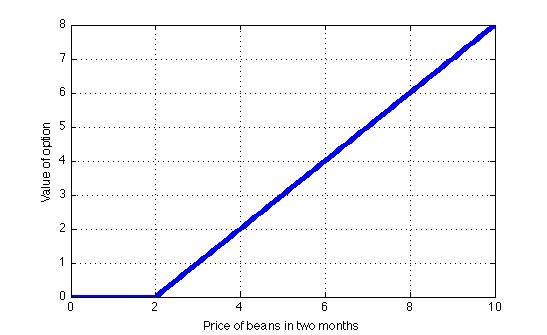
\includegraphics[width=3in]{pics/beanscall.png} 
\end{center}

This type of contract is called a \textbf{call option}. A call option has a \textbf{strike price} (\$2 in example above) and an \textbf{expiry} (two months time). There are also \textbf{put options} which give the option to sell at a certain price. A put option on beans with a strike price of \$2 and a 2 month expiration would look like this:

\begin{center}
  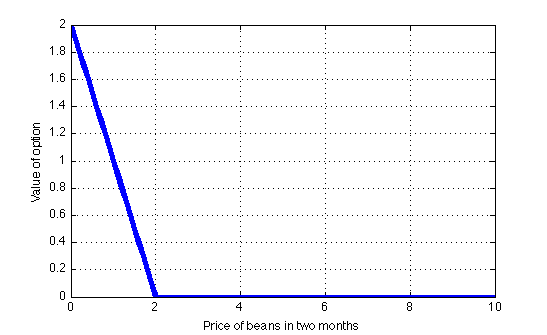
\includegraphics[width=3in]{pics/beansput.png} 
\end{center}


\section{Extracting risk-neutral probabilities from option prices}

Figure \ref{call} is the payoff of a call option to buy something denoted $S$ at a future time $T$:

 \begin{center}
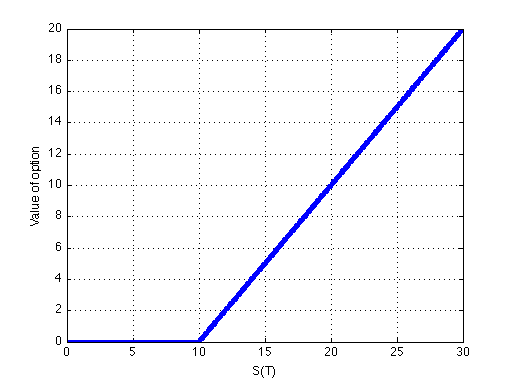
\includegraphics[width=3in]{pics/calloption}%
\captionof{figure}{A call option}\label{call}%
\end{center}

Figure \ref{simple} is the payoff of a simple bet

 \begin{center}
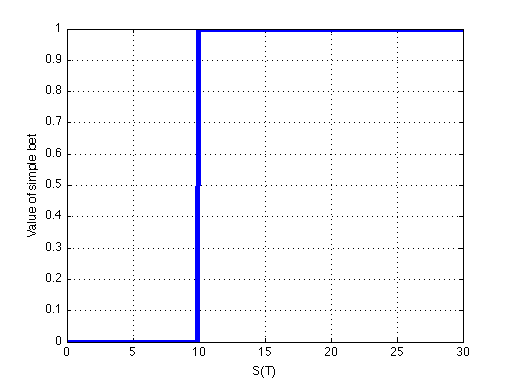
\includegraphics[width=3in]{pics/simplebet}%
\captionof{figure}{A simple bet}\label{simple}%
\end{center}


To construct a simple bet from call options, buy a call option at strike $K$ and sell a call option at  a nearby strike $K+\delta$. The combined portfolio is worth 0 if the price at expiry is less than $K$, $\delta$ if the price is greater than $K+\delta$, otherwise $S(T)-K$.

The value of the security underlying the option will be called $S(t)$. The option expires at time $T>t$. 

\begin{eqnarray*}
\mbox{Bought call at strike $K$ + Sold call at strike $K+\delta$ }&= +C_{K,T}-C_{k+\delta,T}\\
&= 
\begin{cases} 
0 \mbox{ if } & S(T)\leq K \\ 
S(T)-K \mbox{ if} &K < S(T)< S(T)+\delta \\
 \delta \mbox{ if } &S(T)  \geq K+\delta 
 \end{cases} 
 \end{eqnarray*}

The first panel in figure \ref{callToSimple} is the bought call at strike $K$, the second panel is the sold call at strike $K+\delta$. The third panel is the combined payoff. (In this example the first strike is 10 and the second strike is 11 so $\delta = 1$.)
 
 \begin{center}
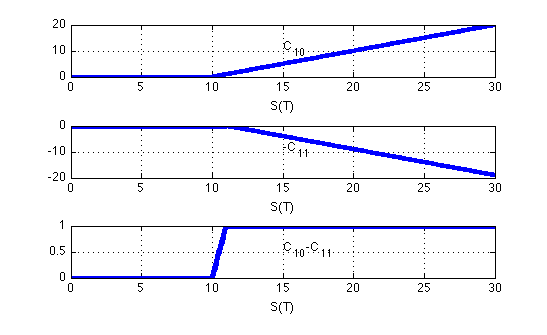
\includegraphics[width=4in]{pics/callspread}%
\captionof{figure}{Constructing a simple bet from call options}\label{callToSimple}%
\end{center}
 

Provided that $\delta$ is small this portfolio is very similar to a simple bet. As $\delta$ approaches 0, it approaches a bet that pays 0 if the price at expiry is less than $K$ and $\delta$  if the price is greater than $K$. If the price of an option at $K$ is $V_{C_{K,T}}$ then the total portfolio costs $V_{C_{K,T}}-V_{C_{K+\delta,T}}$.

Recall in the introduction we established that a bet that pays $Z$ if an event happens and $0$ if it doesn't and costs $a$ implies a probability of $A$

\[P(A) = \frac{a}{Z}\]

In our current example the 'event' $A$ is the price being greater than $K$, and the probability is

\[P(A) = \lim_{\delta \rightarrow 0} \frac{V_{C_{K,T}}-V_{C_{K+\delta,T}}}{\delta} \]

If $C$ is a differentiable function (let's say it is) this is actually just the first derivative of the function $V_{C_{x,T}}$ evaluated at $x=K$

\[ P(A) = \frac{\partial V_{C_{K,T}}}{\partial K} \]

More precisely

\[ P(S(T) \geq K) = \frac{\partial V_{C_{K,T}}}{\partial K}\]

This is a really nice result. It means that if we have option prices for a security at some expiry we have a (risk neutral) probability distribution for the price. If someone asks ``what's the probability that the USD/JPY exchange rate will be above 150 by next year?'' we can give a probability consistent with market prices. It also means that anybody who disagrees with the risk neutral distribution can place a trade against it. This leads to a much richer set of trading strategies than just punting if something will go up or down.

%It's also a good example of the fundamental theorem of arbitrage free prices which says that arbitrage free prices are associated with a unique risk neutral probability distribution. 

\section{How do we get $V_{C_{K,T}(t)}$?}
If we have some function that gives us option prices then we have the risk neutral probability distribution and all is well. But how do we get it? There are two common approaches to explaining option pricing -- both are fairly unintelligible if you don't have a mathematical background. However the basic idea is quite simple. If you can grasp the one big idea it's not so important if you follow the minutiae.


\subsection{The big idea}

We've already seen that there is a relationship between the arbitrage free price and a risk neutral probability. But we don't yet know how to get the correct price. The big idea behind arbitrage free pricing is that the price of an option should be such that we cannot create an arbitrage. We can figure out what the correct price (and probability) is by assuming there is no arbitrage and working backwards.

This is an important idea because it divorces the price of a security from how much a subjective investor might expect it to be worth on average, or how risky it is, or any other consideration. Everything comes down to arbitrage.

The price of the option at time $t$ is given by the value function $V_{C}(t)$. That's what we're making.

%Doing so requires an arbitrage free framework to hedge the instrument: our goal is the price of the hedge is the price of the security. There will be some risk neutral probabilities associated with the correct prices, and we know how to make those from the last section.

%Unfortunately there is no really simple way to describe how these prices and probabilities are obtained. There are intuitive explanations, but they leave a lot of questions. There is an approach which perfectly describes the core process driving the hedge, while actually describing a different kind of hedge. That's a good starting point. It gives the tools to understand the process at play. And stopping there is fine. So is extending the framework to describe the exact type of arbitrage relationship that defines option prices and their associated probabilities.

\subsection{One period, two states}

We'll consider a very simple market with only two possible outcomes. The arbitrage logic in this scenario is the same as in more complicated scenarios. 

\subsubsection{Pricing options by arbitrage}
Suppose we are in a market with an asset priced at $S$. The asset has two possible future states: \textit{up} or \textit{down}. In the up state it's worth $S_u = S(1+u)$, $u>0$; in the down state it's worth $S_d = S(1+d)$, $d<0$ Call options are available for this market. In the 'up' state the call is worth $V_{C_u} = \max(S_u-K,0)$. In the 'down' state it's worth $V_{C_d} = \max(S_d-K,0)$ In this market you can borrow or lend at a rate $r$. We'll impose that $d<r<u$.

Now we construct a portfolio with $h$ shares of the stock and -1 call (so we sell the call). This portfolio will have two possible values depending which state occurs

\begin{eqnarray*}
V_u = hS_u -V_{C_u}\\
V_d = hS_d -V_{C_d}
\end{eqnarray*}

Our strategy will be to make this portfolio worth the same amount in either case. If we achieve that the portfolio will be \textbf{riskless}. A riskless portfolio will only return the risk-free rate $r$, otherwise there would be an arbitrage (we could borrow/lend at $r$ and buy/sell the riskless portfolio).

This is easy:

\begin{eqnarray*}
hS_u -V_{C_u} = V_u = V_d = hS_d - V_{C_d}\\
\rightarrow h = \frac{V_{C_u}-V_{C_d}}{S_u-S_d}
\end{eqnarray*}
 
The portfolio costs $hS-C$. For no-arbitrage to hold the discounted value of both $V_u$ and $V_d$ (they're the same now) must be equal to $hS-V_{C}$. This gives us enough information to solve for $V_{C}$

\begin{eqnarray*}
\frac{hS_u-C_u}{1+r}= hS-V_{C}\\
\rightarrow V_C = \frac{p V_{C_u}  + (1-p) V_{C_d}}{1+r}
\end{eqnarray*}

Where $p = \frac{r-d}{u-d}$. There's a bit of rearranging needed to get this but it's all straightforward (check it yourself). In this form it's also clear that the risk-neutral probability of the 'up' state is $p$. If we substitute back for $p$, $V_{C_u}$ and $V_{C_d}$ we get

\[V_{C} =\frac{r-d}{u-d} (S(1+u)-K)(1+r)^{-1}\]

We could have found the risk neutral probability first and then priced the option. We'll do that in the next section.
 
\textbf{Example:}\\

We'll set up an incorrect call price to create the arbitrage and then solve for the correct price. We face the following two state market:

\begin{itemize}
\item Current price:  $S = 100$
\item Interest rate: $r = 0.25$
\item Up move: u = 2 ($S_u =  S(1+u) = 30$)
\item Down move: d = -0.5 ($S_d = S(1+d) = 5$)
\item Call option strike: $K =10$ 
\item Call price: $V_C = 5$
\end{itemize}


Recall the arbitrage portfolio is short 1 call option and long $h$ units of the stock where $h$ is

\[ h = \frac{V_{C_u} - V_{C_d}}{S_u-S_d} = \frac{20 - 0}{30-5} = 0.8\]

If the \textit{up} state occurs we get $hS_u-V_{C_u} = .8*30-20 = 4$. If the \textit{down} state occurs we get  $hS_d-V_{C_d} = .8*5-0 = 4$. The portfolio costs $hS -V_{C} = .8*10-5 = 3$. If we borrow \$3 now and invest in the portfolio we have to pay back \$3.75. We get an \textbf{arbitrage profit} of .25 no matter what happens.

\begin{center} \begin{tabular}{|c|c|c|}
  \hline
  % after \\: \hline or \cline{col1-col2} \cline{col3-col4} ...
  & \textit{up} & \textit{down}\\
  \hline
  now & borrow \$3 & borrow \$3 \\
           &buy 0.8 units of $S$ &buy 0.8 units of $S$\\
           &sell 1 call & sell 1 call\\
  \hline
  1 year & repay 3*(1+.25) = 3.75 & repay 3*(1+.25) = 3.75\\
              & sell 0.8*30 = 24 & sell 0.8*5 = 4\\
              & pay call (30-10) = 20 & pay call 0\\
  \hline
             & 24-20-3.75 = 0.25 (arbitrage profit) & 4-0-3.75 = 0.25 (arbitrage profit)\\
             \hline
\end{tabular}
\end{center}

The risk-neutral probability is 
\begin{eqnarray*}
p = \frac{r-d}{u-d} =0.3
\end{eqnarray*}

The arbitrage free price is

\begin{eqnarray*}
C = \frac{p V_{C_u}  + (1-p) V_{C_d}}{1+r}\\
 = p(S(1+u)-K)(1+r)^{-1} \\
= 0.3(30-10)(1+0.25)^{-1} = 4.8
\end{eqnarray*}


\subsubsection{The easy way}

We already have the arbitrage free price and the risk neutral probability, but it's interesting and instructive to get it in another way. 

The price $S$ is the discounted expectation of the two states using risk-neutral probabilities. Call the probability of the \textit{up} state $p_u$ and the \textit{down} state $p_d$
 
 \[S = (p_u S_u + p_d S_d)(1+r)^{-1}\]

The price is the discounted expectation under the \textbf{risk neutral} probabilities. Since $p_d = (1-p_u)$, and substituting for $S_u$ and $S_d$ we have

\[S = (p_u S(1+u) + (1-p_u)S(1+d))(1+r)^{-1}  \]

Solving for $p_u$ gives

\[ p_u = \frac{r-d}{u-d}\]
and
\[p_d = \frac{u-r}{u-d} \]

With these risk-neutral probabilities we may price the option. The discounted expected value of a call option with strike $K$ is

\[V_C = (p_u V_{C_u}+ p_d V_{C_d})(1+r)^{-1}\]

Substitute in $C_u = S(1+u)-K$ and $C_d = 0$

\[C = \frac{r-d}{u-d} (S(1+u)-K)(1+r)^{-1}\]

This is the arbitrage free price for the call option in this two-state model. 

Markets with more periods and more states are priced in the same way. First we determine a set of probabilities (or probability distribution) which make the price equal to its discounted expectation \textit{at each point in time}. Then we use those probabilities to price the value of the option by taking the discounted expectation of the value of the call in each scenario.


\section{The real formula}

Real world markets do not have two states and one period. The correct price of an option is generated by a similar process as the two-state model, by ensuring that the probabilities are \textbf{risk neutral} and the price \textbf{arbitrage free} for \textit{every possible state at every possible time}. 

This is not the place to derive these more complicated models. We will simply state without proof that the correct price of a call option for \textbf{continuous time} ($T$ periods, infinitely divisible) with an \textbf{infinite number of possible states} (S can go from 0 to infinity) is

\begin{eqnarray}
V_{C(K,T)}(t) = N(d_1)S - N(d_2)Ke^{-r(T-t)}\\
d_1 = \frac{\ln \frac{S}{K} + r+\frac{\sigma^2}{2}(T-t)}{\sigma \sqrt{T-t}}
d_2 = \frac{\ln \frac{S}{K} + r-\frac{\sigma^2}{2}(T-t)}{\sigma \sqrt{T-t}}
\end{eqnarray}

Where $\sigma$ is the standard deviation of the underlying asset returns\footnote{A return is $r=\log(S(t+1)/S(t))$. This is a random variable and has a standard deviation $\sigma = $}, $t$ is the current time, and $N(.)$ is the cumulative distribution function of the standard normal distribution.\footnote{Which is $\int_{-\infty}^x \frac{1}{2\pi}e^{-\frac{x^2}{2}}dx$}
 
The derivation is a extension of the single-period two-state model, but it uses the central limit theorem and something called It$\hat{o}$ Calculus. 

%If you don't understand the central limit theorem you really should be doing that before worrying about option prices. You should also be worrying about the decisions you've made in life.

\textbf{An incorrect objection}

One objection is that price changes don't follow a normal (Gaussian) distribution, and the formula has the form of a Gaussian distribution in its pricing function. People who make this criticism and don't understand the logic of Black-Merton-Scholes. The central limit theorem says that a sufficiently large number of draws from \textit{any} distribution, no matter how peculiar, will be normally distributed. Black-Merton-Scholes uses this in the derivation. The distribution of price movements doesn't matter provided that it doesn't change. If it does change, the sums aren't from an identical distribution, and so you have to deduce the arbitrage free price in a more complicated way. But if the distribution is constant, then no matter how peculiar, or skewed, or `fat-tailed' the distribution is, Black-Merton-Scholes holds.

%There's another kind of incorrect objection: that options are a \textbf{redundant security}. This claim derives from the fact that in a Black-Merton-Scholes world, you can replicate an option price exactly with an appropriate trading strategy on the underlying security, Therefore in that world there is no need to buy options, you can just make them yourself. That makes them redundant: you could live without them.  

%But in the real world nobody ever knows what the volatility is. An option is implicitly a bet that the volatility of the underlying security will be $\sigma$. There's no other way to bet on volatility. Even if the price dynamics go completely off the rails there's going to be a risk neutral probability distribution. It allows us to answer questions like ``what's the probability that the Google Inc. will trade above 500 in a year's time?" We can't answer that question in an arbitrage free way without options. 

And that's it. That's option pricing. 

\section{What about $P_K$?}

All of this has been about call options. The same arbitrage logic can be used to price put options, but you don't need to worry about the details because the price of call and put options is connected by an arbitrage relationship called \textbf{put-call parity}

\subsection{Put-call parity}

Say we have call and put options both at strike $K$ (first and second panel of figure \ref{comboToFuture}). A portfolio of a call option and a sold put (panel 3) gives us a straight line (panel 4). 

Now if we add a sold future with the same expiry (first panel of figure \ref{comboToArb}) as the call and put (panel 2) we get an unchanging payoff (panel 3). If this line is above zero we have an arbitrage. It follows that if we know the call price and the futures price we can figure out an arbitrage free put price. The details are below

 \begin{center}
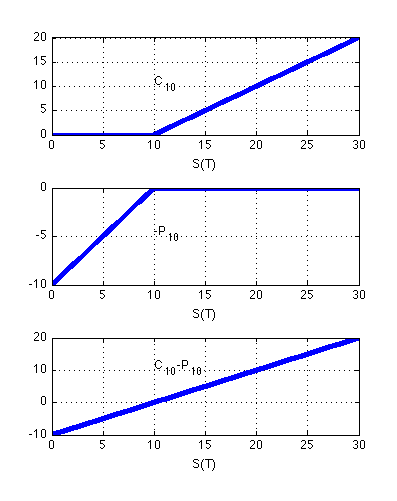
\includegraphics[width=4in]{pics/cpf}%
\captionof{figure}{A bought call plus a sold put is like a future}\label{comboToFuture}%
\end{center}


 \begin{center}
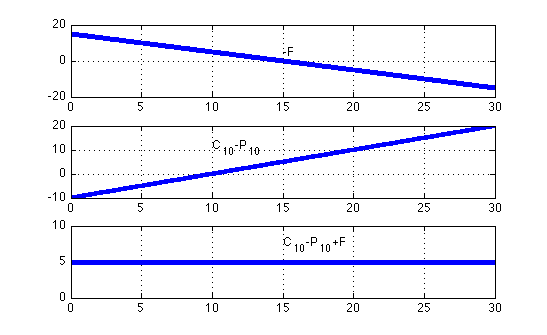
\includegraphics[width=4in]{pics/cpfarb}%
\captionof{figure}{A bought call plus a sold put plus a sold future is an arbitrage}\label{comboToArb}%
\end{center}


\begin{center}
\begin{tabular}{|l|c|}
\hline
now &Borrow/Lend $V_{C_K} - V_{P_K}$\\
	&Buy 1 call for $V_{C_K}$\\
	&Sell 1 put for $V_{P_K}$\\
	&Sell 1 future for F\\
\hline
one year
	       & repay/receive ($V_{C_K}-V_{P_K})(1+r)$\\ 
	       & Receive $(S-K)^+$\\
	       & pay $(K-S)^+$ on the put\\
	       & deliver futures contract for F-S\\
	       \hline
	       &$S-K + (F-S) - (V_{C_K}-V_{P_K})(1+r) = F-K - (V_{C_K}-V_{P_K})(1+r)$\\
	       \hline
\end{tabular}
\end{center}

The no-arbitrage condition is

\begin{eqnarray*}
F-K - (V_{C_K}-V_{P_K})(1+r) \leq 0\\
V_{C_K} - \frac{F-K}{1+r} \geq V_{P_K}
\end{eqnarray*}

The arbitrage works in reverse too (sell the call, buy the put, buy the future) and produces

\[ V_{C_K} - \frac{F-K}{1+r} \leq V_{P_K}\] 

Since it must be both greater than or equal to \textit{and} less than or equal to, it must be equal to

\[ V_{C_K}- \frac{F-K}{1+r} =  V_{P_K}\] 

\section{Questions}

\textbf{Question 1:}\\
An online betting company is offering \$5 for Pakistan to win against India in the cricket. What's the risk-neutral probability of Pakistan winning?

\textbf{Question 2:}\\
A bookie is offering 5:2 odds on for the horse 'Mr Pinkerton" in the third race. What is the risk neutral probability of Mr Pinkerton winning the race?

\textbf{Question 3:}\\
Suppose the price of a call option is given by the function $V_{C_K} = \ln(K)$. What is the probability that the price will be above \$5 at expiry? 


\textbf{Question 4:}\\Suppose the price moves only in increments of \$1. Use the options from question 3 to construct a simple bet that the price will be above \$10 at expiry. What is the arbitrage free price of this bet? What is the risk-neutral probability?


\textbf{Question 5:}\\The following situation prevails in a two-state market
\begin{itemize}
\item Current price:  $S = 10$
\item Up move: u = 6 ($S_u =  S(1+u) = 70$)
\item Down move: d = -1 ($S_d = S(1+d) = 0$)
\item Interest rate: r = 0.25
\item Call option strike: $K =10$ 
\item Call price: $V_C = 5$
\end{itemize}

 \begin{enumerate}
 \item Construct an arbitrage to take advantage of the mispriced call.\\
\item What are the risk-neutral probabilities of the \textit{up} and \textit{down} states.
\end{enumerate}

\textbf{Question 6:}\\A call at a strike of 10 costs \$5. The futures contract trades at $10$. What is the correct price of the put if the interest rate is 25\%?

\textbf{Question 7:}\\
Construct an arbitrage if the put costs \$6


%Consider two investment strategies

%Strategy 1:
%\begin{itemize}
%Start with \$B in cash
%Borrow a further \$R and invest the \$(R+B) in the stock (R = B\frac{1}{\frac{1+r}{1+d}-1})
%\end{itemize}

%Strategy 2:
%Buy $X$ options on the stock ($X = \frac{(B+R)(1+u)-R(1+r)}{Su}$)

%The payoff of strategy in both states is in the table below

%Strat1,u (R+B)(1+u)-(1+r)R
%Strat1,d (R+B)(1+d)-(1+r)R = 0

%Strat2,u X (S(1+u)-S) = XSu = \frac{(B+R)(1+u) - (1+r)R }{Su}Su = (B+R)(1+u) - (1+r)R
%Strat2,d  0 

%Strategy 1 and 2 pay the same amount in either state, they are perfect substitutes so they must have the same price or there will be an arbitrage. Strategy 1 costs \$B, strategy 2 costs \$XC. So it must be that C = B/X. This is the arbitrage free price of the call option.

%Substituting for $X$ gives 

%\begin{eqnarray}
%C = SuB/[(B+R)(1+u) - (1+r)R]
 % =  Su/[(1+R/B)(1+u) - (1+r)R/B]
 % = Su/[(1+\frac{1}{\frac{1+r}{1+d}-1})(1+u) - (1+r)\frac{1}{\frac{1+r}{1+d}-1}]
%\end{eqnarray}

%So the value of the call option is a function of $S$ $u$, $d$, and $r$.

%The risk neutral probability can be making the expected value of a call option equal to zero. If we get the 'up' state we get Su-C and if we get the 'down' state we get -C. So:

%\begin{eqnarray}
%P(u)(Su-C)  + (1-P(u))*-C = 0\\
%\rightarrow P(u) = \frac{Su}{C} =  \frac{(B+R)(1+u)-R(1+r)}{B} = (1+R/B)(1+u)-R/B(1+r)
%\end{eqnarray}

%Substituting for $R$ gives

%\begin{eqnarray}
%P(u) = (1+\frac{1}{\frac{1+r}{1+d}-1})(1+u)-\frac{1}{\frac{1+r}{1+d}-1}(1+r)
%[reduced form]
%\end{eqnarray}

%This is also a simple bet that we know about. It provides a risk-neutral probability and an arbitrage free price with a very simple technique. It has similar qualities as a 'heads or tails' game.

%Here's you:

%(picture)

%and here's your decisions with their possible consequences and probabilities.

%(picture)

%If it goes 'up' the call option gives you a dollar, and you have to pay for the option which is priced \$C, so you get 1-C(1). If the option goes down the option pays nothing but you still have to pay for it so you get $-C(1)$. You can borrow or lend any amount of money at rate $r$.

%In this world you can do a combination trade. If it costs the same to produce two trades and the trades have a different price you have a potential arbitrage, and that's not allowed.
 
%You face the following investment opportunities:

%Strategy 1:


%[example]

%The prices are different if the price of the option is less than or equal to X. The same logic holds if you do the opposite, so it has to be greater than or equal than X. We can deduce that the price must be exactly X. Then we have arbitrage free prices and risk neutral probabilities, we're set. 

%Now you might ask what about if there are another set of prices that are also arbitrage free. What then? That's a stupid question. Intuitively the price and probability must be unique. Otherwise there would be a trivial arbitrage buying one set of prices and selling another. And in that case they wouldn't be arbitrage free. Would they?

%That's it. That's the two-state one-period binomial problem.


%\subsection{}

%What we might want to do is expand this definition by looking at a n-state n-period binomial problem. It looks like this:


